\section{Haptics}

\textit{Importance of haptics}

Haptics is the study of touch, force and tactile feedback in human-computer-interaction. 
Haptics feedback is everywhere and could be used for gaming, robotic surgery, education and many more. 

\begin{itemize}[itemsep=-5pt, topsep=0pt, leftmargin=*]
	\item Enhances user experience and engagement
	\item Enables more intuitive and natural interactions
	\item Adresses limitations of visual and auditory feedback
	\item Vital for accessability and inclusion
\end{itemize}\medskip



\textit{Interaction benefits}  \smallskip
\begin{itemize}[itemsep=-5pt, topsep=0pt, leftmargin=*]
	\item Increased accuracy and speed
	\item Reducing errors
	\item Eyes Free interaction
	\item Proprioceptive
\end{itemize} \medskip

\textit{Tactile} \smallskip

All about vibrations and textures.

\begin{itemize}[itemsep=-5pt, topsep=0pt, leftmargin=*]
	\item Sense of touch
	\item Goal: Stimulate skin in a programmable manner to create desired set of sensations
	\item Tactile feedback is generated by tactile device
	\item Skin based
	\item Examples: Vibration, pain, pressure, temperature
	\item Used in touchscreens, tactile displays and VR
\end{itemize}


\textit{Vibrotactile} \smallskip

\begin{itemize}[itemsep=-5pt, topsep=0pt, leftmargin=*]
	\item Subset of tactile
	\item Relies on vibrations to convey information
	\item Common in mobile devices, notifications and wearables
\end{itemize}


When designing actuators its important to consider thath different cells are in different parts of hand. 
They have different receptive fields and frequency ranges. \smallskip

Limitations of vibrotactile sensation: Broad localization of the sensation, superficial feedback and thus the strength of the vibration may be perceived differentyl based on the area of skin in contact with mounting pressure. 
\medskip

\textit{Kinesthetic} \smallskip

Very accurate receptors in muscles, joint and skin. All about movement and force.  \smallskip

Passive Kinesthetic (Force feedback): Perception of resistance or force, it requires human motion/input. Examples are surgical simulators or controllers. 


Limitations to passive kinesthetic: 


\begin{itemize}[itemsep=-5pt, topsep=0pt, leftmargin=*]
	\item Hard to design
	\item Often cumpersome
	\item User needs to provide inpput
	\item Limited part of how we perceive the world
\end{itemize}


\textit{Active Kinesthetic} \smallskip

Focuses on the sense of body movement and position. Relevant in motion simulators, exoskeletons and teleoperation systems. 


Limitations to passive kinesthetic: 


\begin{itemize}[itemsep=-5pt, topsep=0pt, leftmargin=*]
	\item Hard to design
	\item Often cumpersome
	\item Expensive
	\item Limited part of how we perceive world
\end{itemize} \medskip

\textbf{Current Limitations of Haptics} \smallskip

The chain is: System state triggers an actuator, which in turn is perceived by a human.

Kisthetics are currently not common in user electronics. 

 

\begin{itemize}[itemsep=-5pt, topsep=0pt, leftmargin=*]
	\item Kisthetics are currently not common in user electronics. 
	\item Human state is not taken into account
	\item Current systems only react to system states
	\item We are limited to vibrotactile feedback
	\item This leads to underperforming and underwhelmin feedback
\end{itemize} \medskip


\textbf{How to overcome these limitations?}


\begin{itemize}[itemsep=-5pt, topsep=0pt, leftmargin=*]
	\item Enable sensing of human state
	\item Use human state to control the device intelligently
	\item Using Closed vs open loop
	\item Body pose as a first step for truly intelligent haptic feedback systems
\end{itemize} \medskip

Add control:
\begin{center}
	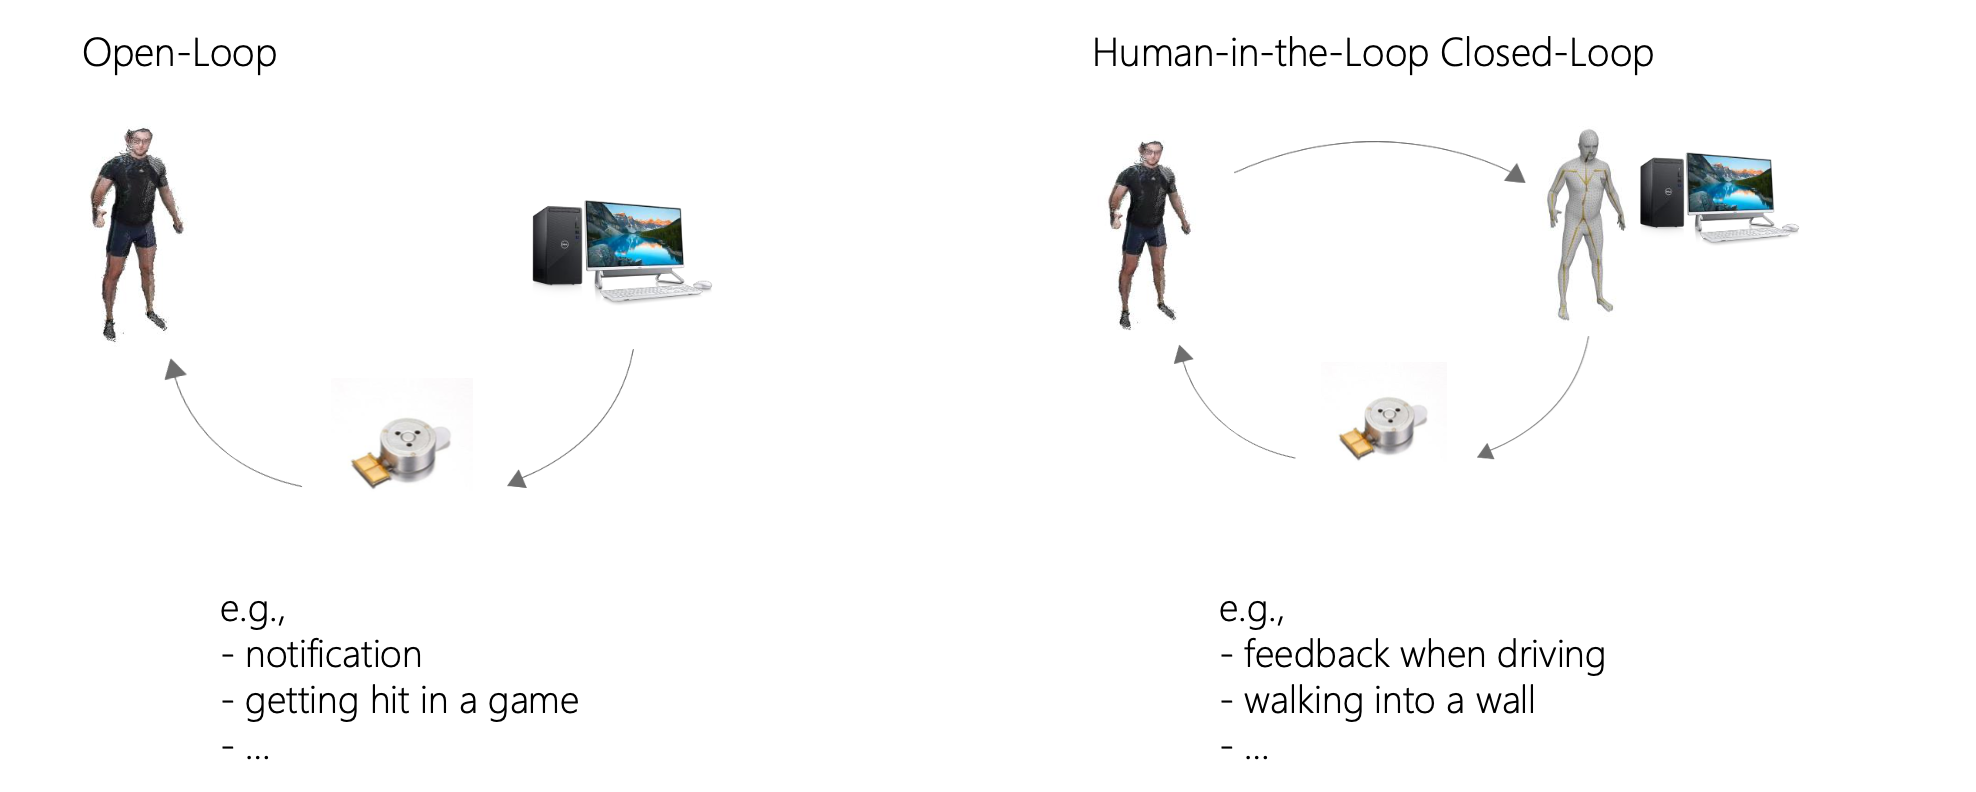
\includegraphics[width=\linewidth]{control.png}
\end{center}

\begin{center}
	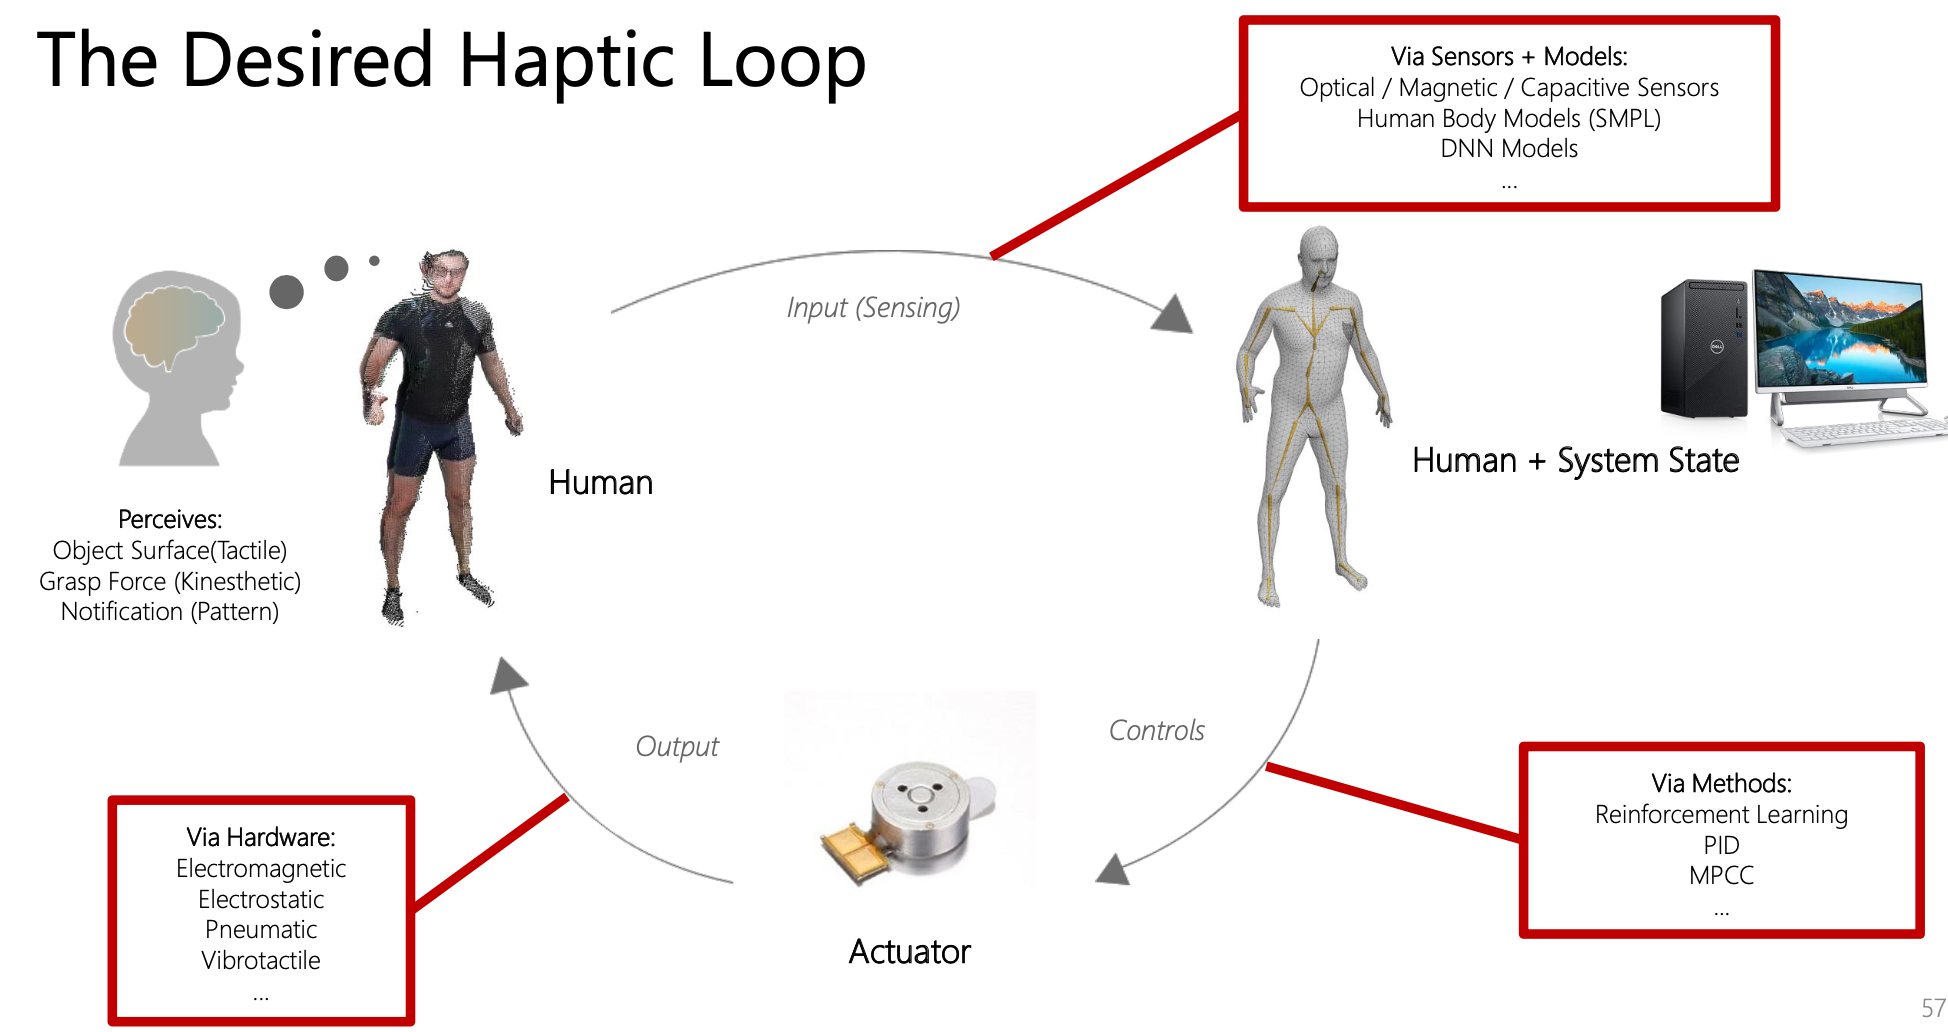
\includegraphics[width=\linewidth]{desired_loop.png}
\end{center}

\medskip

Example of a closed-form solution to calculate electromagnetic force.
\begin{center}
	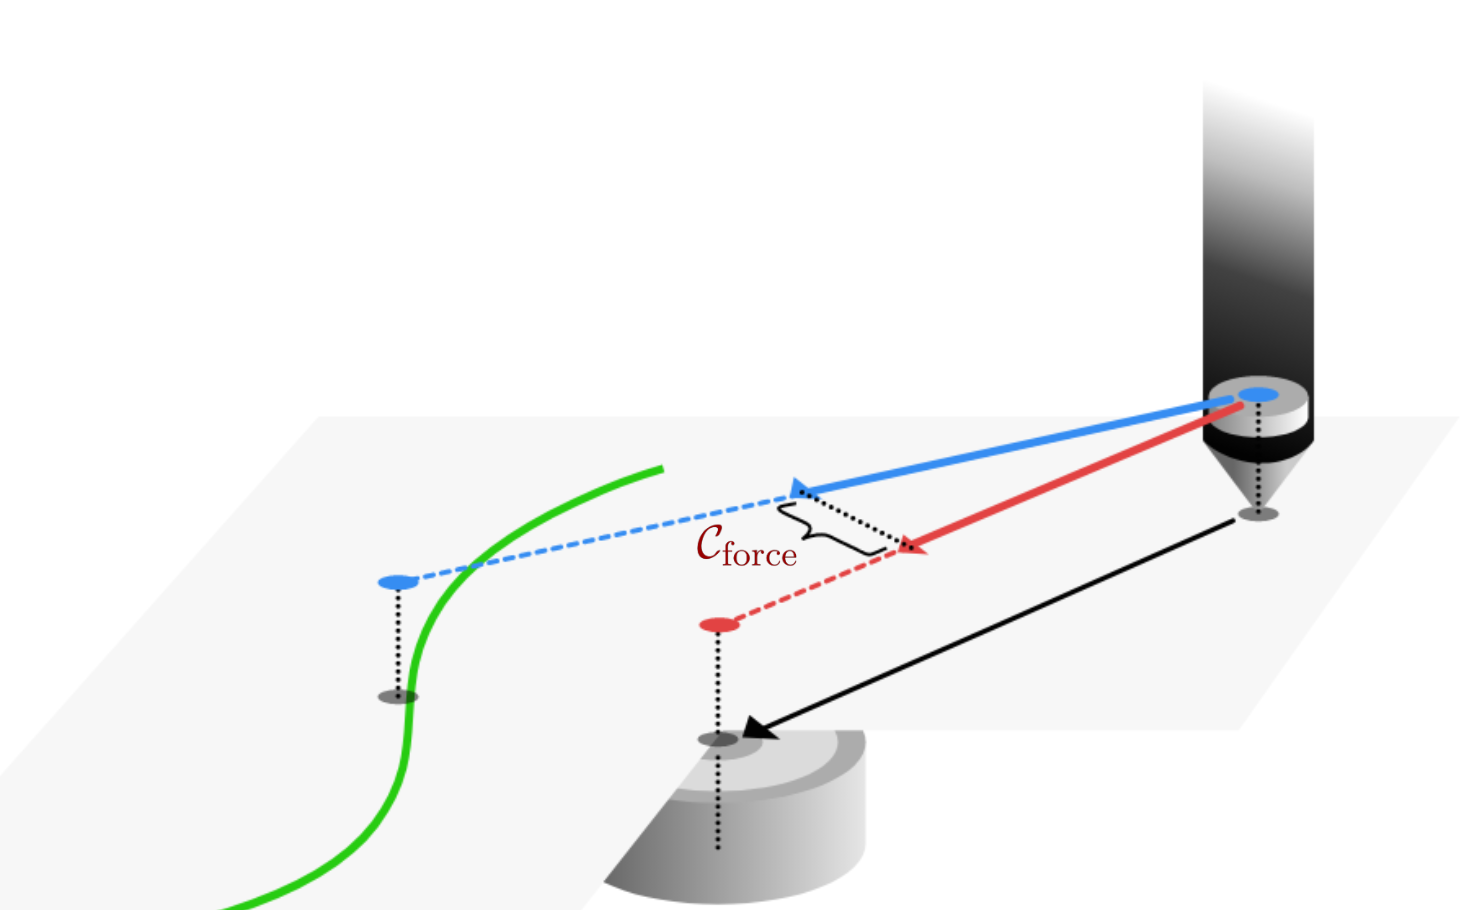
\includegraphics[width=\linewidth]{example_closeloop.png}
\end{center}

It has been found that more complex shapes beenfit most from feedback. And users are still limited by the speed of the system. 
But overall drawings are more accurate that way. 
